\subsection{Decision Theory}
% \begin{figure}[htpb]
%     \centering
%     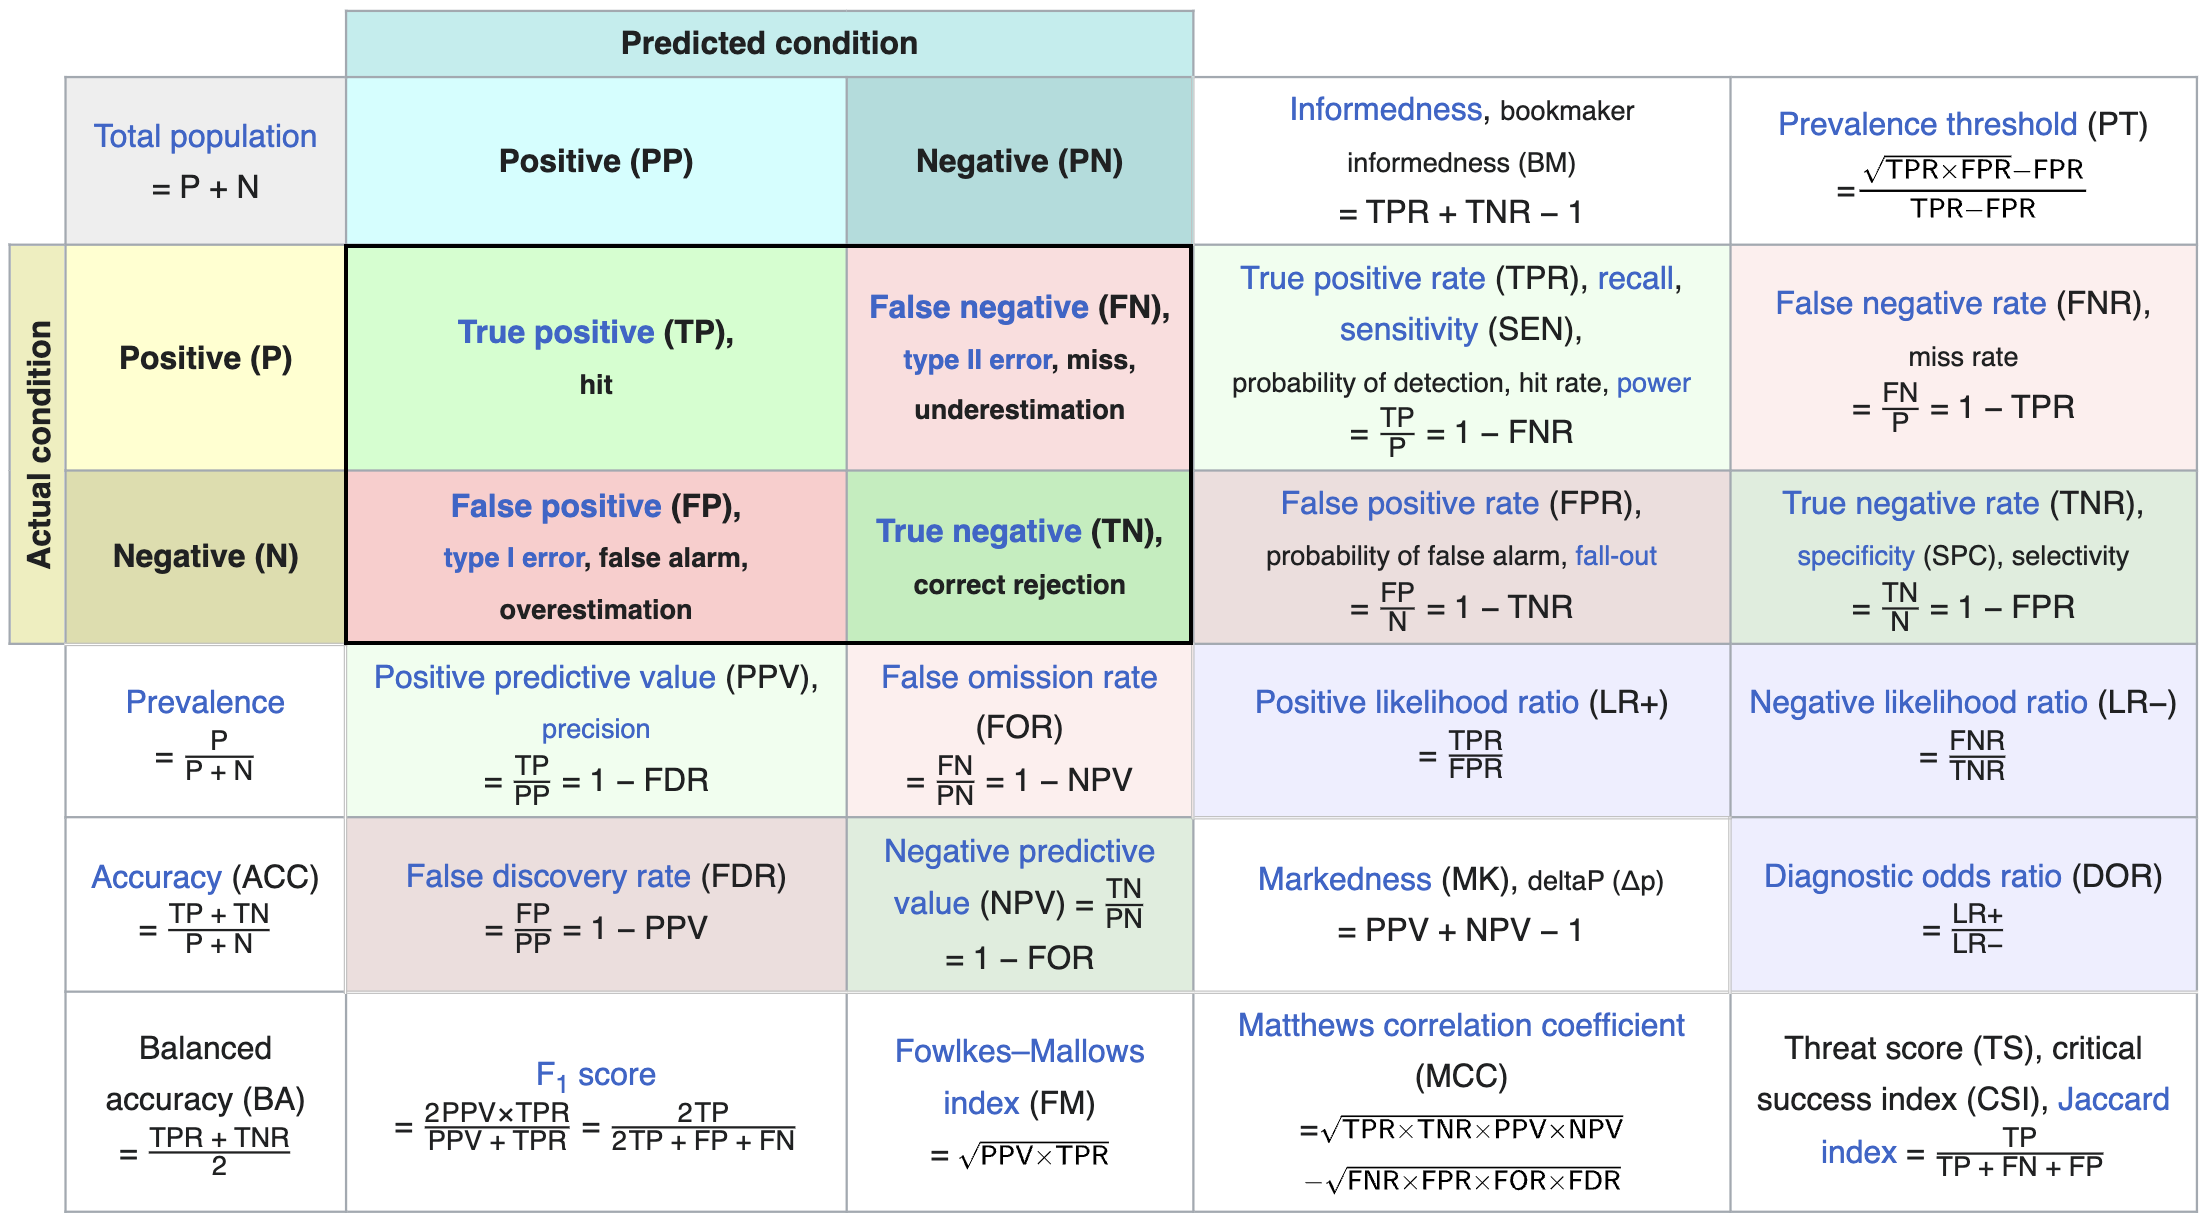
\includegraphics[width=\textwidth]{figs/confusionmtx.png}
%     \caption{Confusion matrix and the metrics defined on it}
%     {\footnotesize This table comes from Wikipedia (https://en.wikipedia.org/wiki/Confusion\_matrix).}
%     \label{fig:confusionmtx}
% \end{figure}

\begin{figure}[htpb]
    \centering
    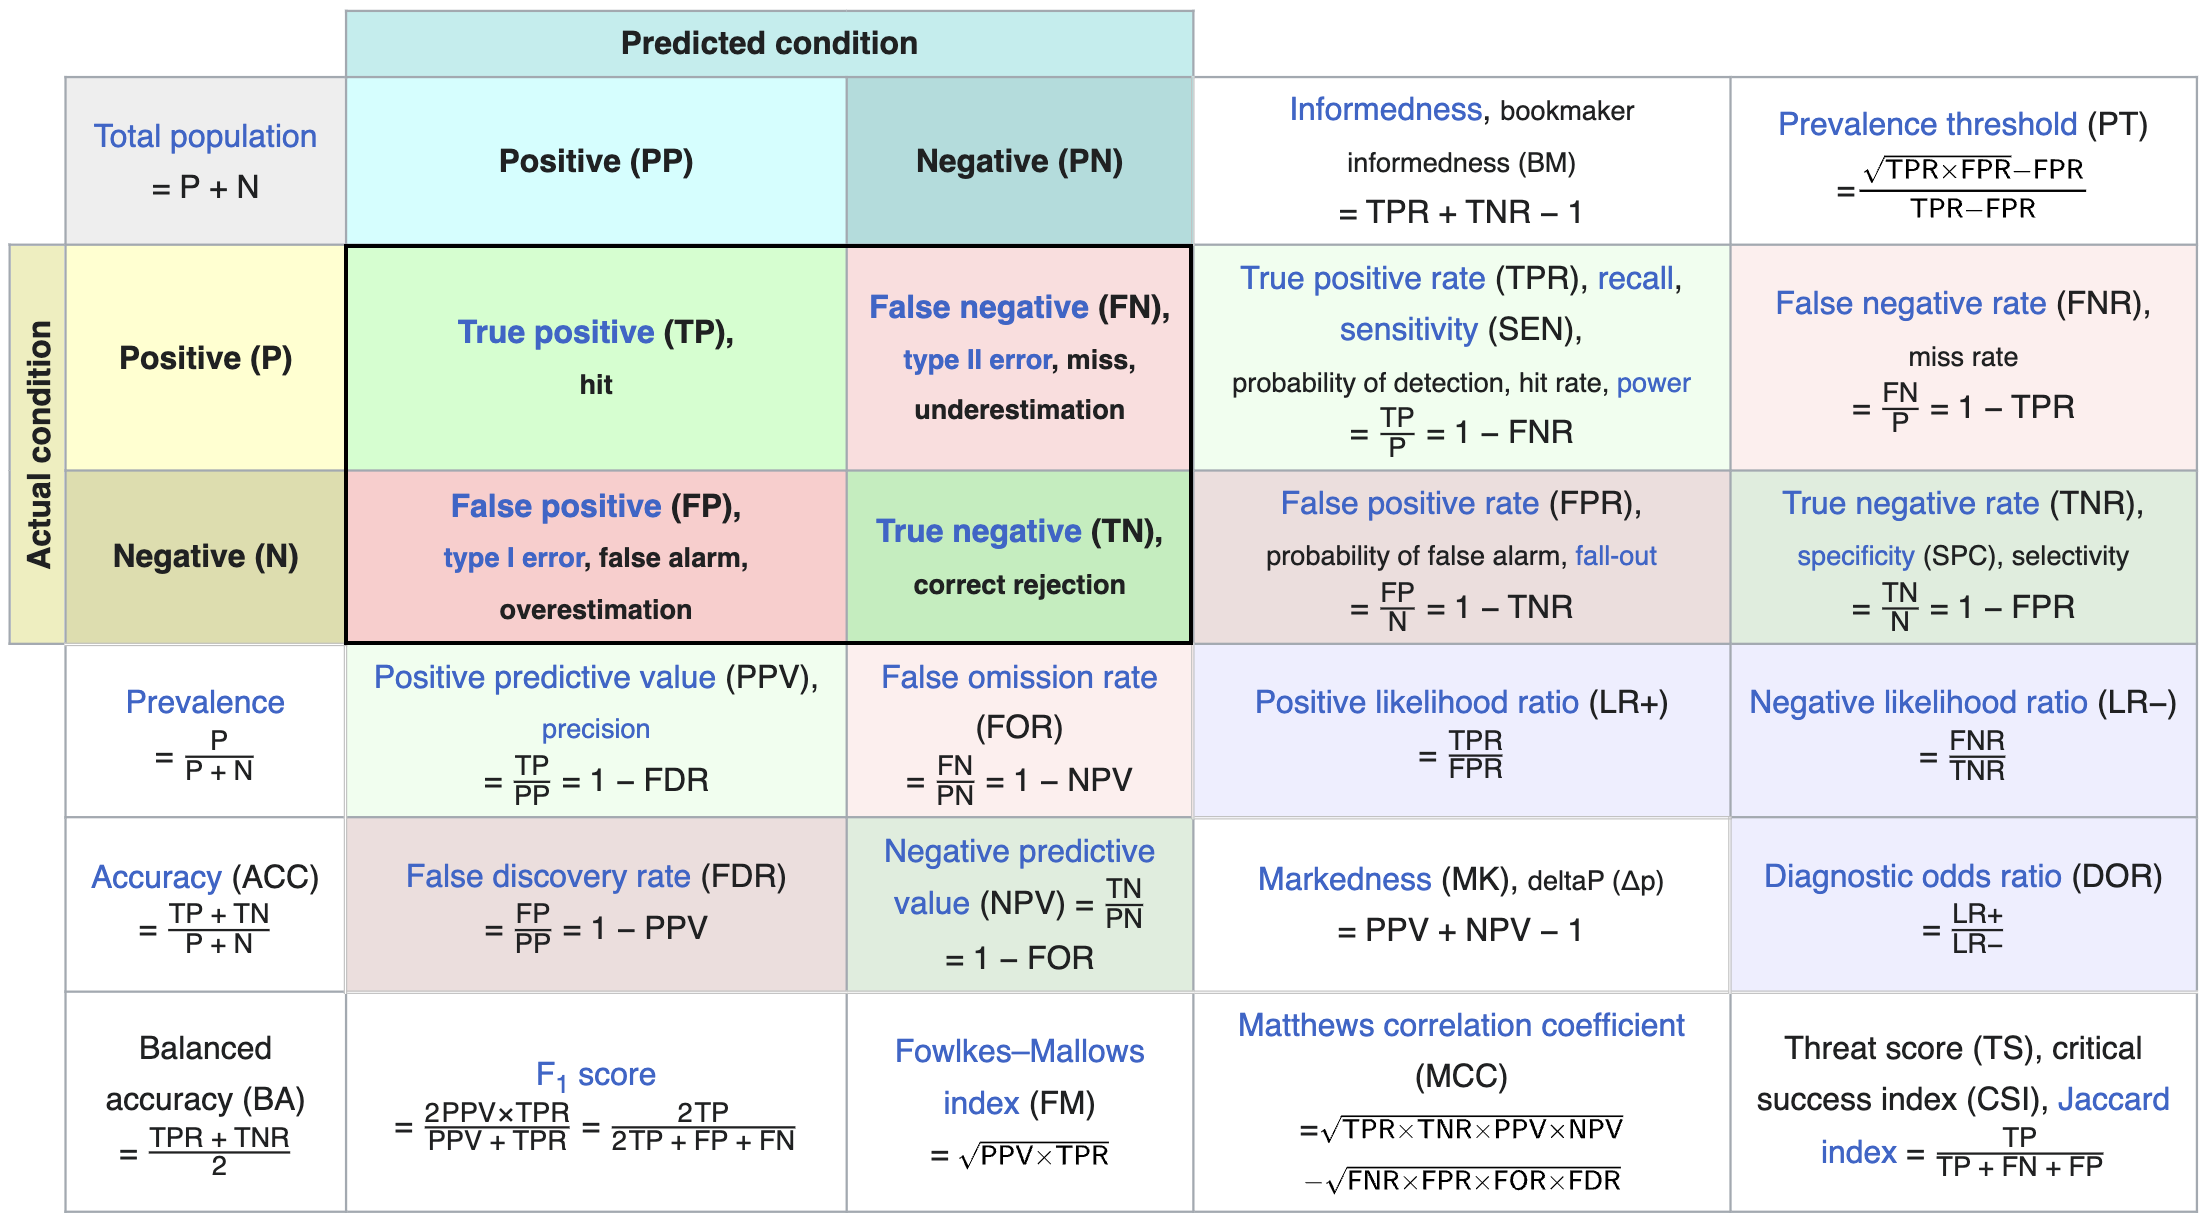
\includegraphics[width=\textwidth]{figs/confusionmtx.png}
    \caption{Confusion matrix and the metrics defined on it}
    {\footnotesize This table comes from Wikipedia (https://en.wikipedia.org/wiki/Confusion\_matrix).}
    \label{fig:confusionmtx}
\end{figure}

\textbf{Receiver operating characteristic (ROC) curves}: 
x-axis: FPR (1-Specificity) and y-axis: TPR (Recall or Sensitivity);
and \textbf{Precision-recall (PR) curves}:
x-axis: Recall and y-axis: Precision.
ROC curves (and the area under it, AUC) will not be unaffected by class imbalance,
while PR curves (and the area under \textit{interpolated} ones, AP) are sensitive to a large change in the absolute number in imbalance problem,
preferable when the shifting of absolute numbers are concerned, such as a ``negative'' is not well-defined.
 
\textbf{Huber loss}: equivalent to $\ell_2$ for errors smaller than $\delta$, 
and $\ell_1$for larger errors.
\begin{gather}
    \ell_\delta(h,a)=\left\{
    \begin{array}{ll}
        \frac{1}{2}(a-h)^2              & \text{if}~|a-h|\leq\delta\\
        \delta|a-h|-\frac{1}{2}\delta^2 & \text{if}~|a-h|>\delta
    \end{array}
    \right.
\end{gather}

\textbf{Kullback Leibler (KL) divergence}:
\begin{align}
    \infdiv{p}{q}
    \triangleq& \sum_{y\in\mathcal{Y}}p(y)\log\frac{p(y)}{q(y)}\\
    =& \underbrace{\sum_{y\in\mathcal{Y}}p(y)\log{p(y)}}_{-\mathbb{H}(p)}
        \underbrace{-\sum_{y\in\mathcal{Y}}p(y)\log{q(y)}}_{\mathbb{H}_\text{ce}(p,q)}.
\end{align}
Minimizing KL divergence between the fixed given $p$ and a $q$ is equal to find a $q$ minimizing the cross-entropy between $p$ and $q$.
$\log{\frac{p()y}{q(y)}}$ term can be quite sensitive to errors for low probability events,
so the \textbf{Brier score} an alternative
\begin{gather}
    \ell(p,q)\triangleq\frac{1}{C}\sum_{c=1}^C[q(y=c|\bm{x})-p(y=c|\bm{x})]^2
\end{gather}

\textbf{Bayes factor} for Bayesian hypothesis testing\unsure{
Recall the definition of marginal likelihood or evidence for a model $m$, 
$p(\mathcal{D}|m)=\int{p(\bm{\theta}|m)p(\mathcal{D}|\bm{\theta},m)}d\bm{\theta}$.
The model presented here is a family of distribution indexed by the parameter $\bm{\theta}$, 
so we need marginal likelihood for an average probability for family $m$ as feasible region of optimization.
}
\begin{gather}
    B_{1,0}\triangleq\frac{p(\mathcal{D}|M_1)}{p(\mathcal{D}|M_0)}
\end{gather}

\begin{table}[htbp]
    \centering
    \begin{tabular}{cl}
    \toprule
    Bayes factor $B_{0,1}$                      & Interpretation \\
    \midrule
    $(0,\frac{1}{100})$                         & Decisive evidence for $M_0$ \\
    $(\frac{1}{100},\frac{1}{10})$              & Strong evidence for $M_0$ \\
    $(\frac{1}{10},\frac{1}{3})$                & Moderate evidence for $M_0$ \\
    $(\frac{1}{3},1)$                           & Weak evidence for $M_0$ \\
    $(1,3)$                                     & Weak evidence for $M_1$ \\
    $(3,10)$                                    & Moderate evidence for $M_1$ \\
    $(10,100)$                                  & Strong evidence for $M_1$ \\
    $(100,\infty)$                              & Decisive evidence for $M_1$ \\
    \bottomrule
    \end{tabular}
    \caption{Jeffreys scale of evidence for interpreting Bayes factors}
    \label{tab:bayesfactor}
\end{table}

\textbf{Information criteria} ($D_m=|\bm{\theta}|$)
\begin{itemize}
    \item \textbf{Bayesian information criterion (BIC)}: 
    Gaussian approximation to the posterior $p(\bm{\theta}|\mathcal{D})$ with the assumptions of 
    {uniform prior ($p(\bm{\theta})\propto 1$) and iid of samples}.
    \begin{align}
        J_\text{BIC}(m)=&\log{p(\mathcal{D}|m)}\approx\log{p(\mathcal{D}|\hat{\bm{\theta}},m)-\frac{D_m}{2}\log{N}}\\
        \Rightarrow
        \mathcal{L}_\text{BIC}(m)=&-2\log{p(\mathcal{D}|\hat{\bm{\theta}},m)+D_m\log{N}}
    \end{align}
    
    \item \textbf{Akaike information criterion (AIC)}: 
    The regularization term independent of $N$ derives from a frequentist perspective.
    \begin{gather}
        \mathcal{L}_\text{AIC}(m)=-2\log{p(\mathcal{D}|\hat{\bm{\theta}},m)+2D_m}
    \end{gather}
    
    \item \textbf{Minimum description length (MDL)}:
    The bit length regularization term ($C(m)=-\log{p(m)}$) comes from the perspectives of communication cost.
    \begin{gather}
        \mathcal{L}_\text{MDL}(m)=-\log{p(\mathcal{D}|\hat{\bm{\theta}},m)+C(m)}
    \end{gather}
    
\end{itemize}

% \begin{figure}[htpb]
%     \centering
%     \begin{figure}[htpb]
    \centering
    \begin{tikzpicture}[->,>=stealth',auto,node distance=3.5em,thick,show background rectangle]
    \tikzstyle{every node}=[font=\small,scale=0.9]
      \node[](anchor){};
      \node[left = of anchor]       (loss)  {$\ell(\theta,\delta(\mathcal{D}))$};
      \node[above = of anchor]          (bayes) {$\rho(\mathcal{D})=\mathbb{E}_{\Theta|\mathcal{D}}\ell(\theta,\delta(\mathcal{D}))$};
      \node[below = of anchor]         (freq)  {$r(\theta)=\mathbb{E}_{\mathcal{D}|\theta}\ell(\theta,\delta(\mathcal{D}))$};
      \node[right = of anchor]         (risk)  {$R(\delta)=\mathbb{E}_{\mathcal{D},\Theta}\ell(\Theta,\delta(\mathcal{D}))$};
      
      \draw[->] (loss.east)  --node[below]{Bayesian}     (bayes.south);
      \draw[->] (loss.east)  --node[above]{Frequentist}  (freq.north);
      \draw[->] (bayes.south) -- (risk.west);
      \draw[->] (freq.north)  -- (risk.west);
    \end{tikzpicture}
    \caption{risk from Bayesian and Frequentist perspective}
    \label{fig:riskbf}
\end{figure}
%     \caption{risk from Bayesian and Frequentist perspective}
%     \label{fig:riskbf}
% \end{figure}

\begin{figure}[htpb]
    \centering
    \begin{tikzpicture}[->,>=stealth',auto,node distance=3.5em,thick,show background rectangle]
    \tikzstyle{every node}=[font=\small,scale=0.9]
      \node[](anchor){};
      \node[left = of anchor]       (loss)  {$\ell(\theta,\delta(\mathcal{D}))$};
      \node[above = of anchor]          (bayes) {$\rho(\mathcal{D})=\mathbb{E}_{\Theta|\mathcal{D}}\ell(\theta,\delta(\mathcal{D}))$};
      \node[below = of anchor]         (freq)  {$r(\theta)=\mathbb{E}_{\mathcal{D}|\theta}\ell(\theta,\delta(\mathcal{D}))$};
      \node[right = of anchor]         (risk)  {$R(\delta)=\mathbb{E}_{\mathcal{D},\Theta}\ell(\Theta,\delta(\mathcal{D}))$};
      
      \draw[->] (loss.east)  --node[below]{Bayesian}     (bayes.south);
      \draw[->] (loss.east)  --node[above]{Frequentist}  (freq.north);
      \draw[->] (bayes.south) -- (risk.west);
      \draw[->] (freq.north)  -- (risk.west);
    \end{tikzpicture}
    \caption{risk from Bayesian and Frequentist perspective}
    \label{fig:riskbf}
\end{figure}

\textbf{Populaton risk}: if the true distribution $p^*{\bm{x}, \bm{y}}$ is known, 
then the risk of an estimator $f$ is 
\begin{gather}
    R(f,p^*)=R(f)\triangleq\mathbb{E}_{p^*(\bm{x},\bm{y})}\ell(\bm{y},f(\bm{x})).
\end{gather}
Of course, $p^*$ is unknown, 
but we can approximate it using the \textit{empirical distribution} with $N$ samples
and get \textbf{empirical risk}\unsure{
This distribution is discrete. 
If there are some new data point $(\bm{x},\bm{y})$ that haven't occur in dataset,
then, $p\mathcal{D}(\bm{x},\bm{y})=0$,
so it will need some smoothing method or, directly, use empirical expectation that averages over the observed data points.
Empirical risk minimization widely applied in training a deep learning model, 
and the hypothesis space $\mathcal{H}$ depends on the architecture of model.
}
\begin{gather}
    p_{\mathcal{D}}(\bm{x},\bm{y})
    \triangleq
    \frac{1}{|\mathcal{D}|}\sum_{(\bm{x}_n,\bm{y}_n)\in\mathcal{D}}\delta(\bm{x}-\bm{x}_n)\delta(\bm{y}-\bm{y}_n) \\
    R(f,\mathcal{D})
    \triangleq
    \mathbb{E}_{p_{\mathcal{D}}(\bm{x},\bm{y})}\ell(\bm{y},f(\bm{x}))=\frac{1}{N}\sum_{n=1}^N\ell(\bm{y}_n,f(\bm{x}_n))\\
    \hat{f}_\mathcal{D}=\argmin_{f\in\mathcal{H}}R(f,\mathcal{D}).
\end{gather}
Due to \uline{approximation of true distribution (from data)} and \uline{limitation of tractable hypothesis space (from model)}, 
there will exist errors between empirically optimal estimator $\hat{f}_\mathcal{D}$ and universally optimal estimator $f^{**}$
\begin{gather}
    f^{**}=\argmin_f R(f),~
    f^*=\argmin_{f\in\mathcal{H}} R(f),~
    f^*_{\mathcal{D}_\text{tr}}=\argmin_{f\in\mathcal{H}}R(f,\mathcal{D}_\text{tr})\\
    \mathbb{E}_{p^*}\left[R(f^*_{\mathcal{D}_\text{tr}})-R(f^{**})\right]
    =\underbrace{R(f^*)-R(f^{**})}_{\mathcal{E}_\text{app}(\mathcal{H})}
    +\underbrace{\mathbb{E}_{p^*}\left[R(f^*_{\mathcal{D}_\text{tr}})-R(f^*)\right]}_{\mathcal{E}_\text{est}(\mathcal{H,\mathcal{D}_\text{tr}})}\\
    % \mathbb{E}_{p^*}\left[R(f^*_{\mathcal{D}_\text{tr}})-R(f^*)\right]
    \mathcal{E}_\text{est}(\mathcal{H,\mathcal{D}_\text{tr}})
    = \mathbb{E}_{p_\text{tr}}\ell{(\bm{y},f^*_{\mathcal{D}_\text{tr}}(\bm{x}))}
    - \mathbb{E}_{p_\text{te}}\ell{(\bm{y},f^*_{\mathcal{D}_\text{tr}}(\bm{x}))} + \varepsilon_\text{gen}
\end{gather}
where 
$\mathcal{E}_\text{app}(\mathcal{H})$ is approximation error, 
$\mathcal{E}_\text{est}(\mathcal{H,\mathcal{D}_\text{tr}})$ is estimation/generalization error,
and $\varepsilon_\text{gen}$ is called generalization gap.

\textbf{Structural risk minimization}: minimized the regularized \textit{population} risk to pick a model of right complexity.
\begin{gather}
    \argmin_\lambda\min_{\bm{\theta}}\{R(\bm{\theta})+\lambda C(\bm{\theta})\}
\end{gather}
The empirical risk ignored the risk caused by unobserved data and underestimates the population risk,
and the minimization regularized empirical risk 
\begin{gather}
    R_\lambda(\bm{\theta},\mathcal{D})\triangleq R(\bm{\theta},\mathcal{D})+\lambda C(\bm{\theta})
\end{gather} 
always results in $\lambda=0$.
\begin{itemize}
    \item \textbf{cross-validation}\unsure{In the context of DL, $\lambda$ may be the number of training epochs.}
    \begin{gather}
        \hat{\bm{\theta}}_\lambda(\mathcal{D}_\text{tr})=\argmin_{\bm{\theta}}R_\lambda(\bm{\theta},\mathcal{D}_\text{tr}) \\
        R_\lambda^\text{val}\triangleq R(\hat{\bm{\theta}}_\lambda(\mathcal{D}_\text{tr}),\mathcal{D}_\text{val}),~\text{and}~
        R_\lambda^\text{cv}\triangleq\frac{1}{K}\sum_{k=1}^K{R(\hat{\bm{\theta}}(\mathcal{D}_{K\setminus k}),\mathcal{D}_k)} \\
        \hat{\lambda}=\argmin_\lambda R_\lambda^\text{cv} \\
        \hat{\bm{\theta}}=\argmin_{\bm{\theta}}R_{\hat{\lambda}}(\bm{\theta},\mathcal{D})
    \end{gather}\unsure{In real application, 
    the K model snapshots with the optimal $\hat{\lambda}$ during training process may be ensembled, 
    such as average the predictions,
    to a final model, instead of retrained on the entire dataset, 
    because of the additional cost in running time and resources of computation or storage.}
    \item \textbf{statistical learning theory}: Theorem \ref{thm:boundgenerror} tells us the gap between 
    empirical risk and population risk has an upper bound with some probability. 
    The prediction by the model that reach the upper bound is called \textbf{probability approximately correct},
    when the hypothesis class $\mathcal{H}$ is \textbf{PAC learnable}. 
\end{itemize}

\begin{theorem}\label{thm:boundgenerror}
    \textbf{{Upper bound of generalization risk}}\\
    For any data distribution $p^*$ and nay dataset $\mathcal{D}$ of size $N$ drawn from $p^*$,
    the probability that the \uline{generalization error of a binary classifier selected from a finite hypothesis class $\mathcal{H}$} 
    will be more that $\epsilon$.
    In the worst case, it is upper bounded as follows:
    \begin{gather}
        P\left(
            \max_{h\in\mathcal{H}}{|R(h)-R(h,\mathcal{D})|}>\epsilon
        \right)
        \leq 2\mathrm{dim}(\mathcal{H})\exp\{-2N\epsilon^2\}
    \end{gather}
    where $R(h,\mathcal{D})=\frac{1}{N}\sum_{n=1}^N \mathbb{I}(f(\bm{x}_n)\neq y_n)$ empirical risk, 
    $R(h)=\mathbb{E}_{p^*(\bm{x},y)}\mathbb{I}(f(\bm{x})\neq y)$ population risk, 
    and $\mathrm{dim}(\mathcal{H})=|\mathcal{H}|$.
    When the hypothesis class is infinite, we take $\mathrm{dim}(\mathcal{H})=\mathrm{dim}_\text{VC}(\mathcal{H})$,
    \textbf{VC dimension}, measuring the degrees of freedom of the hypothesis class.
    
    \textit{Remark}: the more data the less error; the larger hypothesis space the more error.
\end{theorem}


\subsection{Information Theory}

% \begin{figure}[htpb]
%     \centering
%     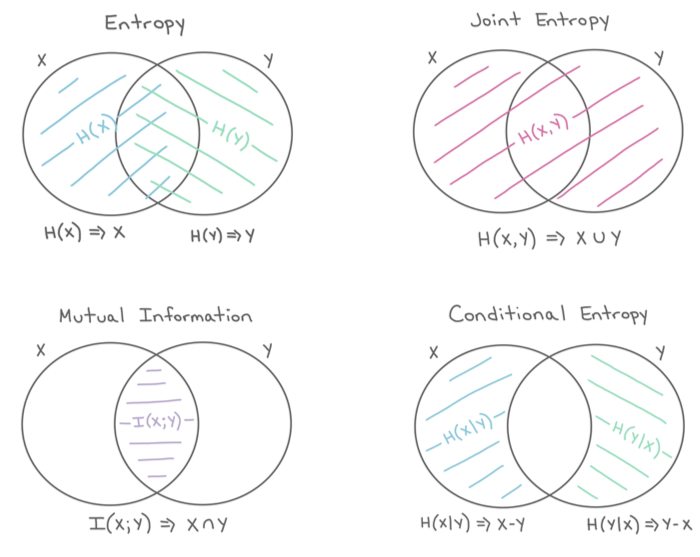
\includegraphics[width=0.6\textwidth]{figs/entropy.png}
%     \caption{The marginal entropy, joint entropy, conditional entropy and mutual information represented as information diagrams.}
%     \label{fig:entropy}
% \end{figure}

\begin{figure}[htpb]
    \centering
    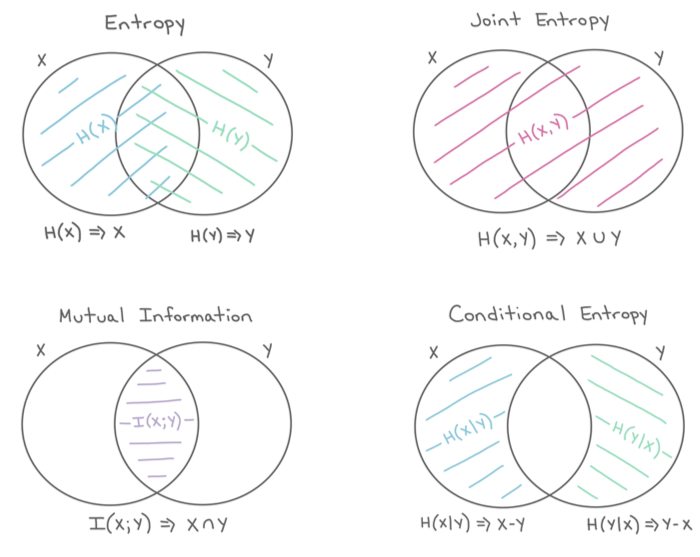
\includegraphics[width=0.6\textwidth]{figs/entropy.png}
    \caption{The marginal entropy, joint entropy, conditional entropy and mutual information represented as information diagrams.}
    \label{fig:entropy}
\end{figure}

\textbf{Cross entropy}: expected number of bits needed to compress some data
samples drawn from distribution $p$ using a code based on distribution $q$,
and the optimal code is reached by $q=p$, i.e., the entropy of $p$ \textbf{(Shannon's source coding theorem)}.
\begin{gather}
    \mathbb{H}(p,q)\triangleq-\sum_{k=1}^K p_k\log_2{q_k}\ge\mathbb{H}(p)
\end{gather}
The continuous version is called \textbf{differetial entropy}
\begin{gather}
    h(X)\triangleq-\int_{\mathcal{X}}p(x)\log{p(x)}dx,
\end{gather}
which can be negative and 
all real-valued quantities can be \uline{represented to finite precision}, 
says, \uline{$n$-bit} \textbf{quantization}, \unsure{Note it is not $B$-bin}
and the approximated discrete value's entropy will be $h(X)+n$. 
One simple approach to discretize is to bin the distribution based on its \uline{empirical quantiles} and the number of bins is determined by 
\begin{gather}
    B=N^\frac{1}{3}\frac{\max{D}-\min{D}}{3.5\sigma_\mathcal{D}}.
\end{gather}

\textbf{Joint entropy} of two random variables $X$ and $Y$
\begin{gather}
    \mathbb{H}(X,Y)=-\sum_{x\in\mathcal{X},y\in\mathcal{Y}}p(x,y)\log_2 p(x,y)\\
    0 \leq \max\{\mathbb{H}(X),\mathbb{H}(Y)\} \leq \mathbb{H}(X,Y) \leq \mathbb{H}(X) + \mathbb{H}(Y)
\end{gather}
where the right equality holds if $X$ \rotatebox{90}{$\models$} $Y$,
which says combining variables together does not make the entropy go down: you cannot
reduce uncertainty merely by adding more unknowns to the problem, you need to observe some data,
and if there is no information introduced by the additional unknowns, the system will reach the maximum chaos.

\textbf{Conditional entropy} of $Y$ given $X$ is the uncertainty we have in $Y$ after seeing $X$, averaged
over possible values for $X$
\begin{align}
    \mathbb{H}(Y|X)
    =& -\sum_{x\in\mathcal{X}}p(x)\sum_{y\in\mathcal{Y}}p(y|x)\log{p(y|x)} \\
    =& -\sum_{x\in\mathcal{X},y\in\mathcal{Y}}p(x,y)\log{\frac{p(x,y)}{p(x)}} \\
    =& \mathbb{H}(X,Y)-\mathbb{H}(X)
\end{align}
\begin{gather}
    0 \leq \mathbb{H}(Y|X) \leq \mathbb{H}(Y)
\end{gather}
where the left equality holds if $Y=f(X)$ where $f$ is deterministic, 
and the right equality holds if $X$ \rotatebox{90}{$\models$} $Y$,
which says that, \textit{on average}, conditioning on data never increases one’s uncertainty.
\begin{gather}
    \mathbb{H}(X_1,\cdots,X_n)=\sum_{i=1}^n{\mathbb{H}(X_i|X_1,\cdots,X_{i-1})}
\end{gather}

\textbf{Relative entropy} or KL divergence\unsure{
already introduced in Chapters 2 and 5.
} measures the (asymmetric) distance between two distributions, which can be interpreted as a lower bound on the number of bits (or ``extra number of bits'') needed to compress data coming from distribution $p$ based on $q$ as the basis of coding scheme.
\begin{align}
    \infdiv{p}{q}
    \triangleq& \sum_{y\in\mathcal{Y}}p(y)\log\frac{p(y)}{q(y)}\\
    =& \sum_{y\in\mathcal{Y}}p(y)\log{p(y)} -\sum_{y\in\mathcal{Y}}p(y)\log{q(y)} \\
    =& -\mathbb{H}(p) + \mathbb{H}_\text{ce}(p,q)
\end{align}

\begin{corollary}
    \textbf{Uniform distribution maximizes the entropy}\\
    $\mathbb{H}(X)\leq\log{|\mathcal{X}|}$, where $|\mathcal{X}|$ is the number of states for $X$, with equality iff $p(x)$ is uniform.
\end{corollary}
\begin{proof}
    Let $u(x)=\frac{1}{|\mathcal{X}|}$, then
    \begin{gather}
        0\leq\infdiv{p}{u}=\sum_{x\in\mathcal{X}}p(x)\log{\frac{p(x)}{q(x)}}=\log{|\mathcal{X}|-\mathbb{H}(X)}
    \end{gather}
\end{proof}

\textbf{Mutual information} measures the dependence of two random variables or the similarity of two distributions, which can serve as a generalized correlation coefficient
\begin{gather}
    \mathbb{I}(X;Y)\triangleq\infdiv{p(x,y)}{p(x)p(y)}
    =\sum_{x\in\mathcal{X}}\sum_{y\in\mathcal{Y}}p(x,y)\log\frac{p(x,y)}{p(x)p(y)}\geq 0
\end{gather}
where the right equality holds iff $X\vperp Y$ and MI approaches $\infty$ if $Y$ tells us an infinite amount of information about $X$.
\begin{align}
    \mathbb{I}(X;Y)
    =& \mathbb{H}(X)-\mathbb{H}(X|Y) \\
    =& \mathbb{H}(Y)-\mathbb{H}(Y|X) \\
    =& \mathbb{H}(X,Y)-\mathbb{H}(X|Y)-\mathbb{H}(Y|X) \\
    =& \mathbb{H}(X) + \mathbb{H}(Y) - \mathbb{H}(X,Y)
\end{align}
\textbf{Conditional mutual information} is the extra information that 
$X$ tells us about $Y$, excluding what we already knew about $Y$ given $Z$ alone.
\begin{align}
    \mathbb{I}(X;Y|Z)
    \triangleq& \mathbb{E}_{p(z)}[\mathbb{I}(X;Y)|Z] \\
    =& \mathbb{E}_{p(z,y,z)}\frac{p(x,y|z)}{p(x|z)p(y|z)} \\
    =& \mathbb{I}(Y;X,Z)-\mathbb{I}(Y;Z)
\end{align}
\textbf{Normalized mutual information (NMI)}: normalize the MI into $[0,1]$, served as ``modern correlation coefficient''
\begin{gather}
    \mathrm{NMI}(X,Y)=\frac{\mathbb{I}(X;Y)}{\min\{\mathbb{H}(X),\mathbb{H}(Y)\}}\in[0,1]
\end{gather}
which need a \uline{discretization technique} to make the \uline{computation tractable}:
\textbf{Maximal information coefficient}
\begin{gather}
    \mathrm{MIC}(X,Y)=\max_{G}\frac{I((X,Y)|_G)}{\log\|G\|}\approx\mathrm{NMI}(X,Y)
\end{gather}
where $G$ is a set of 2D grids, $(X,Y)|_G$ represents a 2D discretization of $X$ and $Y$,
$\|G\|\triangleq\min\{G_x,G_y\}$, $G_x$ is the number of grid cells in the $x$ direction, so be $G_y$.

\begin{theorem}
    \textbf{Data processing inequality}\\
    Suppose $X\to Y\to Z$ forms a Markov chain, so that $X\vperp Z|Y$.
    Then $\mathbb{I}(X;Y)\geq\mathbb{I}(X;Z)$.
\end{theorem}
\begin{proof}
    \begin{align}
        \mathbb{I}(X;Y,Z)
        =& \mathbb{I}(X;Z)+\mathbb{I}(X;Y|Z)\\
        =& \mathbb{I}(X;Y)+\mathbb{I}(X;Z|Y)
    \end{align}
    \begin{gather}
        X\vperp Z|Y\Rightarrow \mathbb{I}(X;Z|Y)=0\\
        \Rightarrow \mathbb{I}(X;Z)+\underbrace{\mathbb{I}(X;Y|Z)}_{\geq 0}=\mathbb{I}(X;Y) \\
        \Rightarrow \mathbb{I}(X;Y)\geq\mathbb{I}(X;Z)
    \end{gather}
    Similarly,
    \begin{gather}
        \mathbb{I}(Y;Z)\geq\mathbb{I}(X;Z)
    \end{gather}
\end{proof}
